\documentclass[a4paper,12pt,twocolumn]{article}
\usepackage{geometry}
\geometry{margin=0.5in}
\usepackage[utf8]{inputenc}
\usepackage[most]{tcolorbox}
\usepackage{chemmacros}
\usepackage{graphicx}
\usepackage[version=4]{mhchem}
\usepackage{nopageno}
\usepackage{tikz}
\usetikzlibrary{calc,intersections,decorations.markings}
\usepackage{enumitem}
\usepackage{subfig}

\colorlet{mylightred}{red!10}
\colorlet{mylightblue}{blue!20}
\newtcolorbox{Box1}[2][]{
                lower separated=false,
                colback=white!80!gray,
colframe=white, fonttitle=\bfseries,
colbacktitle=white!50!gray,
coltitle=black,
enhanced,
attach boxed title to top left={xshift=0.5cm,yshift=-2mm},
title=#2,#1}


\newtcolorbox{Box2}[2][]{
                lower separated=false,
                colback=white,
colframe=black,fonttitle=\bfseries,
colbacktitle=black,
coltitle=white,
enhanced,
attach boxed title to top left={yshift=-0.1in,xshift=0.15in},
                 boxed title style={boxrule=0pt,colframe=white,},
title=#2,#1}

\newtcolorbox{Box3}[2][]{
                lower separated=false,
                colback=white!80!gray,
colframe=white!20!black,fonttitle=\bfseries,
colbacktitle=white!30!gray,
coltitle=black,
enhanced,
attach boxed title to top left={xshift=0.5cm,
        yshift=-2mm},
title=#2,#1}

\newtcolorbox{Box4}[2][]{arc=0mm,
                lower separated=false,
                colback=white!80!gray,
colframe=white!20!black,fonttitle=\bfseries,
colbacktitle=white!30!gray,
coltitle=black,
enhanced,
attach boxed title to top left={xshift=0.5cm,
        yshift=-2mm},
title=#2,#1}

\newcommand{\oxi}[2]{%
    \stackrel{#1}{\mathrm{#2}}
}%
\DeclareUnicodeCharacter{2212}{-}

\begin{document}

\begin{center}
\huge{Phase Rule}
\end{center}

\section{Heterogeneous Equilibria}
\begin{itemize}
\item \textbf{Heterogeneous Systems:} Liquid -vapor, solid -liquid etc. 
\item \textbf{Phase Equilibria:} Heterogeneous equilibria existing between two or more different phases are known as phase equilibria.
\item \textbf{Phase Diagram:} The conditions of equilibria between the various phases of a substance can be represented simultaneously on a single graph which is known as a phase diagram. A phase diagram summarizes the conditions at which a substance exists as a solid, liquid, or gas.
\end{itemize}

\section{Phase Rule}
\begin{itemize}
\item Heterogeneous equilibria or phase equilibria may be described in terms of a very important and exact generalization known as the \textbf{phase rule}.
\item The rule is based purely on \textbf{thermodynamics} and is applicable to all \textbf{macroscopic systems involving heterogeneous equilirbria.} It is independent of atomic or molecular structure. When properly applied to system at true equilibria, the rule gives clearly and unequivocally the maximum number of phase that co-exist under a set of conditions and puts a limit to the variables of the systems such as temperature, pressure, concentration, etc. 
\end{itemize}

\section{Limitations}
\begin{itemize}
\item Phase rule does not consider the effect of gravitation, electrical and magnetic fields, and surface forces. 
\item The rule also does not say anything about the time required for a certain reaction to be complete or the time required for the attainment of equilibrium. 
\end{itemize}

\section{Gibbs Phase Rule}
\begin{itemize}
\item The phase rule discovered by William Gibbs (1874) can be mathematically stated as \\follows: $$\mathrm{F = C - P + 2}$$
where $\mathrm{F}$ is the number of degrees of freedom, $\mathrm{C}$ is the number of components and $\mathrm{P}$ is the number of phases.
\item For applications in materials science dealing with phase changes between different solid structures, pressure is often imagined to be constant (for example at one atmosphere), and is ignored as a degree of freedom. The phase rule for such systems assumes the form $\mathrm{F = C - P + 1}$, as 1 is subtracted from the original equation F = C-P+2, to account for the vapor phase, which is not considered. Such systems are said to be \textbf{condensed systems}. 
\end{itemize}

\section{Definition of Terms:\\ Phase (P)}
\begin{itemize}
\item A phase may be defined as the homogeneous part of a heterogeneous system which is physically and chemically  different from other parts of the same system and bounded by surfaces of separation and mechanically separable.
\item A system can consist of one or more phases:
    \begin{enumerate}
    \item \textbf{One phase systems}
    \item \textbf{Two phase systems}
    \item \textbf{Three phase systems}
    \end{enumerate} 
\end{itemize}

\section{One Phase Systems}
\begin{itemize}
\item A pure substance in one physical state 
\item A mixture of liquids that are completely miscible with each other in all proportions is one phase in the liquid state, e.g., $\ce{H2O / Alcohol}$ 
\item A pure gas or a mixture of gases that do not react with each other 
\item A solution of a solid in a liquid, $\ce{NaCl / H2O}$, $\ce{Sugar / H2O}$, etc 
\item A mixture of solids in the molten state 
\end{itemize}

\section{Two Phase Systems}
\begin{itemize}
\item A pair of immiscible liquids, e.g., $\ce{CCI4/H2O}$, $\ce{C2H2Cl2/H2O}$, etc 
\item A liquid and its vapor 
\item A solid substance and its liquid phase or vapor phase
\item A mixture of solids in the liquid (molten) phase and one of the solids in the solid phase
\item A mixture of two solids which do not react with each other
\end{itemize}

\section{Three Phase Systems}
\begin{itemize}
\item A pure substance existing in three phases together e.g. ice, water, and water vapor 
\item A solid in two allotropic forms and the liquid mixture or in the vapor phase 
\item A mixture of two solids in the molten form and the two solids 
\end{itemize}

\section{Definition of Terms: \\ Component (C)}
\begin{itemize}
\item The number of component is defined as the minimum number of independently variable chemical entities required to describe all parts of a system. 
\item These chemical entities may undergo chemical reaction or physical changes or both, with an increase or decrease of different entities; the number of phases may also change depending on the nature of the changes. 
\item To define the equilibrium conditions of the system it will not be necessary to consider all the chemical entities.
\item There can be systems of one, two or more components. 
\end{itemize}

\section{One Component Systems}
\begin{itemize}
\item \textbf{Water:} Water may exist in three different phases, solid, liquid and vapor. In each case the chemical entity is $\ce{H2O}$. 
\item \textbf{Sulphur:} Sulphur can exist in four phases - two allotropes.
\begin{enumerate}
\item monoclinic (s)
\item rhombic (s), as a liquid and as vapor.
\end{enumerate}
In all these phases the chemical constituent is the same. 
\end{itemize}

\section{Two Component Systems}
\begin{itemize}
\item If $\ce{CaCO3}$ is heated in a closed container it undergoes dissociation forming: $\ce{CaO}$ and $\ce{CO2}$. When the system attains equilibrium all three chemical substances are present. These three chemical entities are related by the equation:
$$\ce{CaCO3 (s) -> CaO (s) + CO2 (g)}$$
There will be three phases, each of the chemical entities representing a phase they are bounded by a separate boundary, but the number of components will be two because all the three phases can be described by mentioning any two of them as they are related by the above equation. 
\item A solution of $\ce{NaCl}$ is a one phase system. The number of components in the system is, however, two as the concentration can vary and the composition of the system cannot be described by mentioning anyone of them. Similarly the number of components in a saturated solution of the salt is also two for the same reason. 
\item Systems in which salts form one or more hydrates are two component systems as the composition of all phases (hydrate ) and water can be described by the constituents, e.g. the salt and water.
\item Pairs of partly miscible or immiscible liquids
\item Pairs of metals which are miscible in the liquid phase but form separate pure solid metal phases
\end{itemize}

\section{Definition of Terms: \\ Degrees of Freedom (F)}
\begin{itemize}
\item The number of degrees of freedom (or variance) may be defined as the number of independent variables e.g. temperature, pressure and composition, which must be fixed in order to define the system completely.
\item Classification:
    \begin{enumerate}
    \item A system with F = 2 is called \textbf{bivariant} 
    \item A system with F = 1 is called \textbf{univariant}
    \item A system with F = 0 is called  \textbf{invariant/nonvaraint}
    \end{enumerate}
\end{itemize}

\section{Degrees of Freedom-Examples}
\begin{enumerate}
\item \textbf{A gaseous system} The temperature, pressure and volume of a gas are related by an equation of state, $\mathrm{PV = RT}$. The state of the gaseous system is completely defined by any two of the three variables. The third is automatically fixed. This is a \textbf{bivariant system}. i.e., the degree of freedom is two. 
\item \textbf{Liquid-vapour system:} The liquid-vapor system has two phases, but one degree of freedom. The vapor pressure is fixed at a definite temperature and does not depend on the quantity of liquid present. Alternatively, one can say the vapor pressure fixes the temperature, i.e., the system is \textbf{univariant}. 
\item \textbf{Solid-liquid-vapour system:} Let us consider the ice-water-vapor system. This is a one-component and three-phase system. All three phases can exist at equilibrium only at a definite temperature and pressure. if anyone of the two variables is changed, the equilibrium is destroyed. So the system has no degree of freedom. i.e. it is a \textbf{nonvariant} system.
\end{enumerate}

\section{Phase Diagram of One Component Systems: Water}
\begin{figure}[h]
    \centering
    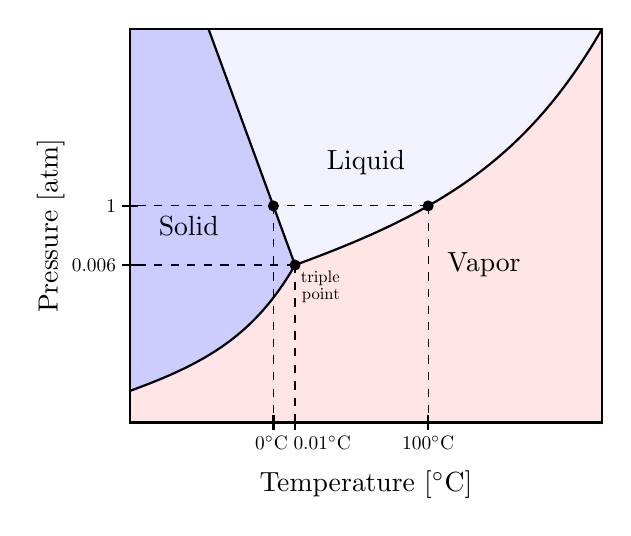
\begin{tikzpicture}[scale=0.5]
      \def\xtick#1#2{\draw[thick] (#1)++(0,.2) --++ (0,-.4) node[below=-.5pt,scale=0.7] {#2};}
      \def\ytick#1#2{\draw[thick] (#1)++(.2,0) --++ (-.4,0) node[left=-.5pt,scale=0.7] {#2};}
      
      % COORDINATES
      \coordinate (O) at (0,0);
      \coordinate (Q) at (0,0.8);
      \coordinate (N1) at (2,10);
      \coordinate (N2) at (11,10);
      \coordinate (NE) at (12,10);
      \coordinate (NW) at (0,10);
      \coordinate (SE) at (12,0);
      \coordinate (W) at (0,5);
      \coordinate (S) at (6,0);
      \coordinate (C) at (12,10); % critical
      \coordinate (T) at (4.2,4); % triple
      
      % PATHS
      \def\SL{(T) -- (N1)}
      \def\SG{(Q) to[out=20,in=-120] (T)}
      \def\LG{(T) to[out=20,in=-120] (C)}
      \def\atm{(0,5.5) -- (12,5.5)}
      \path[name path=SL] \SL;
      \path[name path=LG] \LG;
      \path[name path=atm] \atm;
      
      % REGIONS
      \fill[mylightblue] \SG -- (N1) -- (NW) -- cycle;
      \fill[blue!5] \LG -- (N2) -- (N1) -- cycle;
      \fill[mylightred] \LG -- (N2) -- (NE) -- (SE) -- (O) --  \SG -- cycle;
      \node at (1.5,5) {Solid};
      \node at (9,4) {Vapor};
      \node at (6,6.6) {Liquid};
      
      %% MIXED
      %\shade[top color=mylightblue,bottom color=mylightred,shading angle=70]
      %  (10.4,7.7) -- (11.2,10) -- (10.8,10) -- (10.0,7.7) -- cycle;
      
      % POINTS
      \fill[black,name intersections={of=SL and atm,by=M}] (M) circle (4pt);
      \fill[black,name intersections={of=LG and atm,by=B}] (B) circle (4pt);
      \fill (T) circle (4pt) node[below right,scale=0.6,align=right] {triple\\[-2pt]point};

      
      % LINES
      \draw[thick] \SG;
      \draw[thick] \LG;
      \draw[thick] \SL;
      \draw[dashed] (M) -- ($(M |- 0,0)$) coordinate (Mx);
      \draw[dashed] (T) -- ($(T |- 0,0)$) coordinate (Tx);
      \draw[dashed] (T) -- ($(T -| 0,0)$) coordinate (Ty);
      \draw[dashed] (B) -- ($(B |- 0,0)$) coordinate (Bx);
      \draw[dashed] (B) -- ($(B -| 0,0)$) coordinate (By);

      
      % AXES
      \draw[thick] (O) rectangle (NE);
      \node[left=20pt,above,rotate=90] at (W) {Pressure [atm]};

      \node[below=14pt] at (S) {Temperature [\si{\degree C}]};
      \xtick{Mx}{\hspace{-2pt}0\si{\degree C}}
      \xtick{Tx}{\hspace{28pt}0.01\si{\degree C}}
      \ytick{Ty}{0.006}
      \xtick{Bx}{100\si{\degree C}}
      \ytick{By}{1}
    \end{tikzpicture}
    \end{figure}
    \begin{figure}[h]
    \caption{The phase diagram of water. Each solid line between two phases specifies the conditions of pressure and temperature under which the two phases can exist in equilibrium. The point at which all three phases can exist in equilibrium (0.006 atm and 0.01°C) is called the \textbf{triple point.}}
\end{figure}

\begin{figure}[h]
\centering
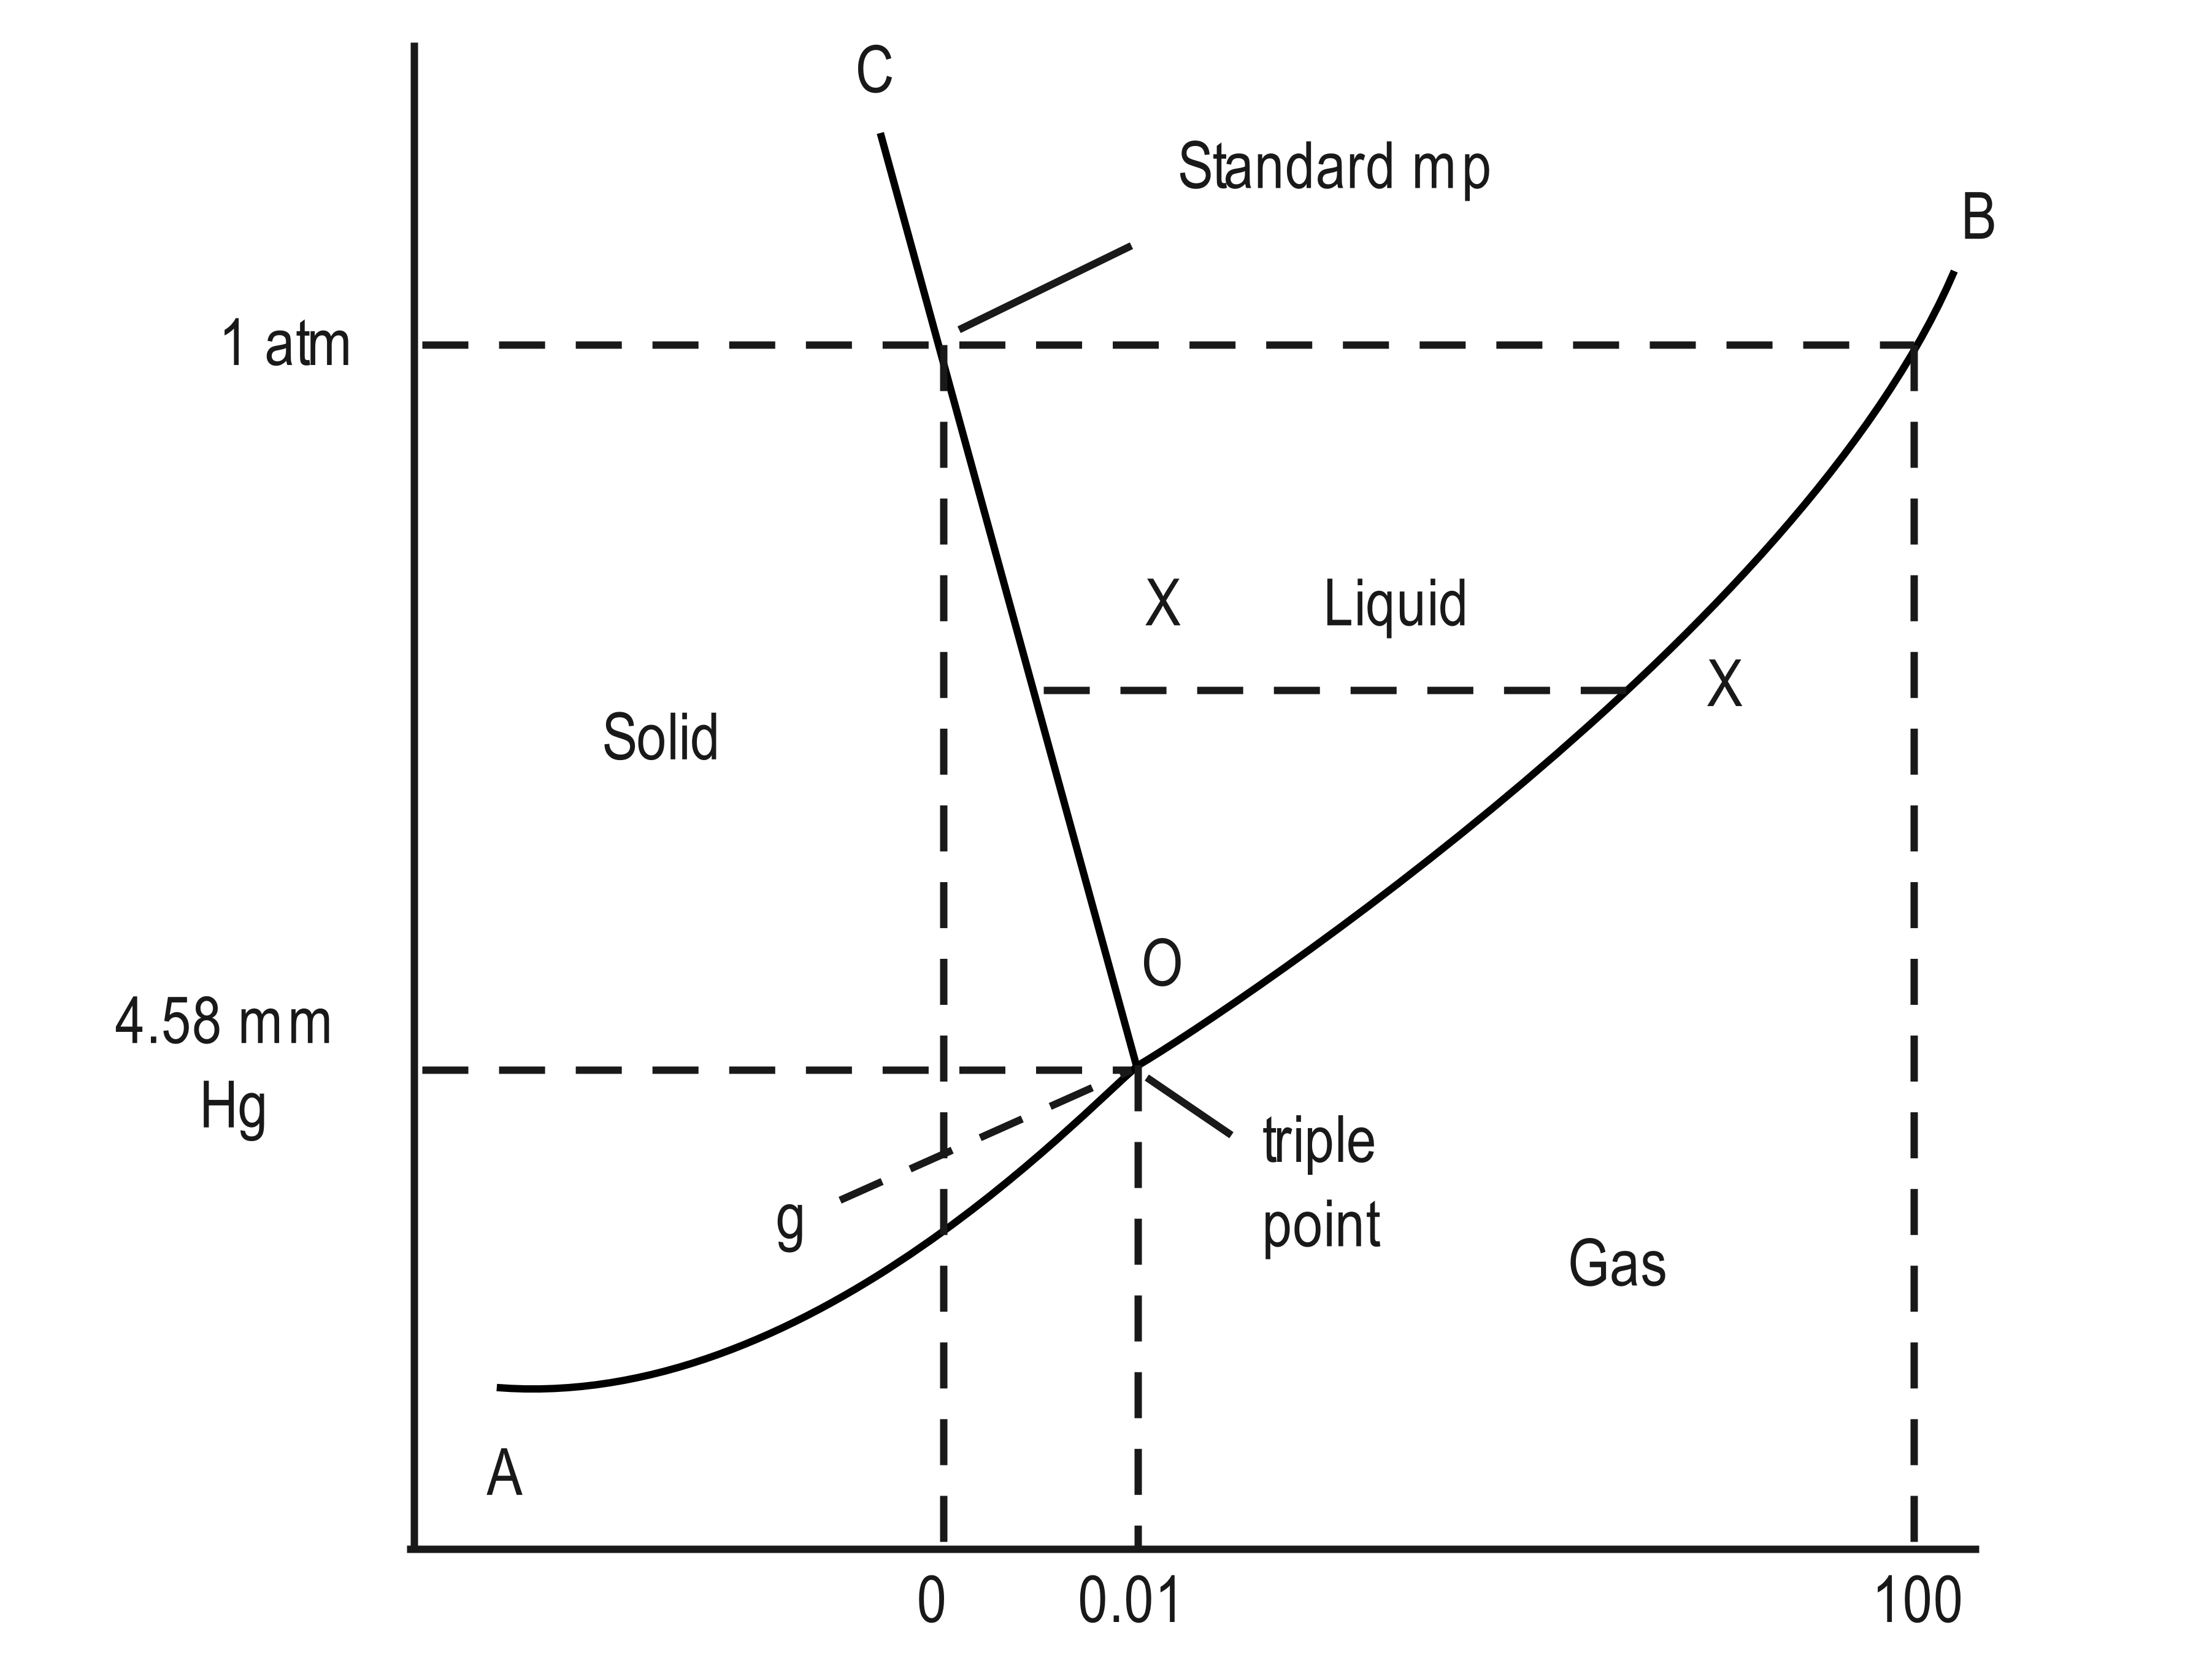
\includegraphics[width=.5\textwidth]{phaseDiagram}
\caption{Phase diagram for water}
\end{figure}

\begin{itemize}
\item The different parts of the diagram are:
    \begin{enumerate}[label=(\alph*)]
    \item Curves OB, OC and OA 
    \item Area within BOC, to the right of BOA and to the left of AOC 
    \item The point O where the three curves OA, OB and OC meet.
    \end{enumerate}
\item The curve OB shows the effect of temperature on the vapour pressure of water. Any point on the curve OB gives the temperature and pressure at which liquid water and vapour co-exist. Since there are two phases in equilibrium the number of degree ($\mathrm{F =1 -2 + 2 =1}$), i.e. the system is \textbf{univariant}, meaning that any of the two variables, temperature and pressure will describe the system. The limit of this curve to the lower temperature side will be the point O, the freezing point of water. 
\item Similarly, the system is \textbf{univariant} along the line OC as any point on the curve gives the temperature and pressure at which solid and liquid water co-exist. The line OC represents the change in the freezing point of water or melting point of ice on changing the pressure.
\item Along the line OA the system is \textbf{univariant} as any point on the line gives the temperature and pressure at which solid and vapour are in equilibrium. The point on the lines OA and OC can be defined by temperature or pressure curve since there are two phases. The curve OA shows the vapour pressure of ice as a function of temperature. Above this curve there is only solid phase and below only vapour. This is, therefore, the sublimation curve of ice. 
\item Area within BOC describes the liquid phase (water), in the area to the right of BOA water is in the form of vapour and the area to the left of AOC is the region where solid phase (ice) exist . The number of degrees of freedom for the component water in all three regions is two (F = 1 -1 + 2 = 2). i e. the system is \textbf{bivariant} in these areas. To describe the system at any point within these regions both temperature and pressure have to be stated. 
\item Along OB liquid and vapor co-exist. Along OC solid (Ice) and liquid co-exist and along OA solid (ice) and vapor (steam) co-exist. These three curves meet at O. Hence at the point O all three phases -solid, liquid and vapor -co-exist or are In equilibrium. This point is called the \textbf{triple point}.  A triple point is, therefore. a point denoted by a definite pressure and temperature at which three phases of a component can co-exist under equilibrium condition. At the triple point $\mathrm{F = 0 (\text{ since } F = 1 -3 + 2 =0)}$; the system is \textbf{Invariant}. This means for the equilibrium between three phases the temperature and pressure are fixed. For water, this point is at \textbf{0.01°C} and \textbf{0.006 atm}.
The curve Og shows the vapor pressure of \textbf{supercooled water} which is a metastable (unstable) slate. The vapor pressure of supercooled water is always greater than the vapor pressure of lce.  In fact, all \textbf{metastable phases} have higher vapor pressure than the stable phase. 
\end{itemize}

\section{Boiling Point and Melting Point}
\begin{itemize}
\item Phase diagrams enable us to predict changes in the melting point and boiling point of a substance as a result of changes in the external pressure; we can also anticipate directions of phase transitions brought about by changes in temperature and pressure. 
\item The normal melting point and boiling point of water at 1 atm are 0°C and 100°C, respectively. 
\end{itemize}

\begin{Box1}{}
What would happen if melting and boiling were carried out at some other pressure? 
\end{Box1}
Increasing the pressure above 1 atm will raise the boiling point and lower the melting point. A decrease in pressure will lower the boiling point and raise the melting point.

\section{Phase Diagram of Water- Effect of Pressure}
\begin{figure}[h]
    \centering
    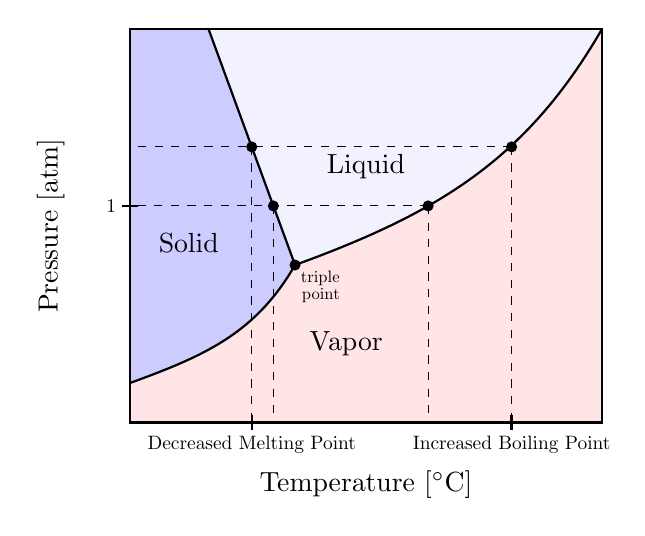
\begin{tikzpicture}[scale=0.5]
      \def\xtick#1#2{\draw[thick] (#1)++(0,.2) --++ (0,-.4) node[below=-.5pt,scale=0.7] {#2};}
      \def\ytick#1#2{\draw[thick] (#1)++(.2,0) --++ (-.4,0) node[left=-.5pt,scale=0.7] {#2};}
      
      % COORDINATES
      \coordinate (O) at (0,0);
      \coordinate (Q) at (0,1);
      \coordinate (N1) at (2,10);
      \coordinate (N2) at (11,10);
      \coordinate (NE) at (12,10);
      \coordinate (NW) at (0,10);
      \coordinate (SE) at (12,0);
      \coordinate (W) at (0,5);
      \coordinate (S) at (6,0);
      \coordinate (C) at (12,10); % critical
      \coordinate (K) at (3.1,7);
      \coordinate (T) at (4.2,4); % triple
      \coordinate (N) at (9.7,7);

      % PATHS
      \def\SL{(T) -- (N1)}
      \def\SG{(Q) to[out=20,in=-120] (T)}
      \def\LG{(T) to[out=20,in=-120] (C)}
      \def\atm{(0,5.5) -- (12,5.5)}
      \path[name path=SL] \SL;
      \path[name path=LG] \LG;
      \path[name path=atm] \atm;
      
      % REGIONS
      \fill[mylightblue] \SG -- (N1) -- (NW) -- cycle;
      \fill[blue!5] \LG -- (N2) -- (N1) -- cycle;
      \fill[mylightred] \LG -- (N2) -- (NE) -- (SE) -- (O) -- \SG -- cycle;
      \node at (1.5,4.55) {Solid};
      \node at (5.5,2) {Vapor};
      \node at (6,6.5) {Liquid};
      
      %% MIXED
      %\shade[top color=mylightblue,bottom color=mylightred,shading angle=70]
      %  (10.4,7.7) -- (11.2,10) -- (10.8,10) -- (10.0,7.7) -- cycle;
      
      % POINTS
      \fill[black,name intersections={of=SL and atm,by=M}] (M) circle (4pt);
      \fill[black,name intersections={of=LG and atm,by=B}] (B) circle (4pt);
      \fill (K) circle (4pt) node[above=1pt,scale=0.6,align=center] {};
      \fill (N) circle (4pt) node[above=1pt,scale=0.6,align=center] {};
      \fill (T) circle (4pt) node[below right,scale=0.6,align=right] {triple\\[-2pt]point};

      
      % LINES
      \draw[thick] \SG;
      \draw[thick] \LG;
      \draw[thick] \SL;
      \draw[dashed] (M) -- ($(M |- 0,0)$) coordinate (Mx);
      \draw[dashed] (B) -- ($(B |- 0,0)$) coordinate (Bx);
      \draw[dashed] (B) -- ($(B -| 0,0)$) coordinate (By);
      \draw[dashed] (N) -- ($(N -| 0,0)$) coordinate (Ny);
      \draw[dashed] (N) -- ($(N |- 0,0)$) coordinate (Nx);
      \draw[dashed] (K) -- ($(K |- 0,0)$) coordinate (Kx);
      % AXES
      \draw[thick] (O) rectangle (NE);
      \node[left=20pt,above,rotate=90] at (W) {Pressure [atm]};

      \node[below=14pt] at (S) {Temperature [\si{\degree C}]};
      \xtick{Nx}{Increased Boiling Point}
      \xtick{Kx}{Decreased Melting Point}
      \ytick{By}{1}

    \end{tikzpicture}
    \caption{The phase diagram of water. This phase diagram tells us that increasing the pressure on ice lowers its melting point and that increasing the pressure of liquid water raises its boiling point.}
\end{figure}

\section{Phase Diagram of One Component Systems: $\ce{CO2}$}
\begin{figure}[h]
    \centering
    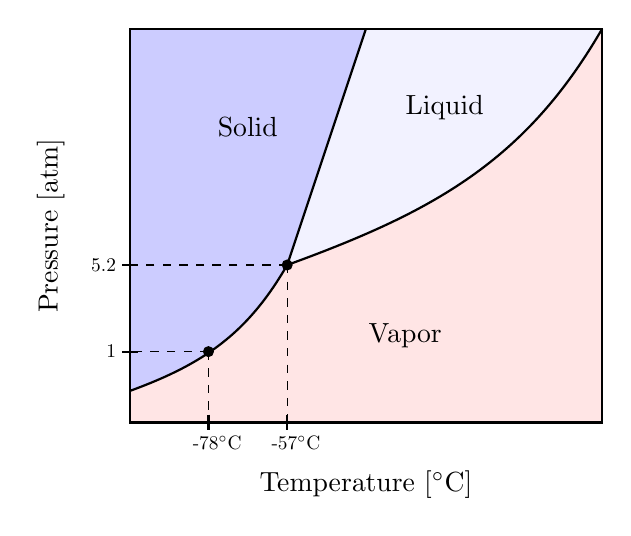
\begin{tikzpicture}[scale=0.5]
      \def\xtick#1#2{\draw[thick] (#1)++(0,.2) --++ (0,-.4) node[below=-.5pt,scale=0.7] {#2};}
      \def\ytick#1#2{\draw[thick] (#1)++(.2,0) --++ (-.4,0) node[left=-.5pt,scale=0.7] {#2};}
      
      % COORDINATES
      \coordinate (O) at (0,0);
      \coordinate (Q) at (0,.8);
      \coordinate (N1) at (6,10);
      \coordinate (N2) at (11,10);
      \coordinate (NE) at (12,10);
      \coordinate (NW) at (0,10);
      \coordinate (SE) at (12,0);
      \coordinate (W) at (0,5);
      \coordinate (S) at (6,0); 
      \coordinate (C) at (12,10); % critical
      \coordinate (T) at (4,4); % triple
      \coordinate (P) at (2,1.8);
      % PATHS
      \def\SL{(T) -- (N1)}
      \def\SG{(Q) to[out=20,in=-120] (T)}
      \def\LG{(T) to[out=20,in=-120] (C)}
      \def\atm{(0,5.5) -- (12,5.5)}
      \path[name path=SL] \SL;
      \path[name path=LG] \LG;
      \path[name path=atm] \atm;
      
      % REGIONS
      \fill[mylightblue] \SG -- (N1) -- (NW) -- cycle;
      \fill[blue!5] \LG -- (N2) -- (N1) -- cycle;
      \fill[mylightred] \LG -- (N2) -- (NE) -- (SE) -- (O) --  \SG -- cycle;
      \node at (3,7.5) {Solid};
      \node at (7,2.2) {Vapor};
      \node at (8,8) {Liquid};
      
      %% MIXED
      %\shade[top color=mylightblue,bottom color=mylightred,shading angle=70]
      %  (10.4,7.7) -- (11.2,10) -- (10.8,10) -- (10.0,7.7) -- cycle;
      
      % POINTS
      \fill (T) circle (4pt) node[below right,scale=0.6,align=right] {};
      \fill (P) circle (4pt) node[below right,scale=0.6,align=right] {};
      
      % LINES
      \draw[thick] \SG;
      \draw[thick] \LG;
      \draw[thick] \SL;
      \draw[dashed] (T) -- ($(T |- 0,0)$) coordinate (Tx);
      \draw[dashed] (T) -- ($(T -| 0,0)$) coordinate (Ty);
      \draw[dashed] (P) -- ($(P |- 0,0)$) coordinate (Px);
      \draw[dashed] (P) -- ($(P -| 0,0)$) coordinate (Py);
      
      % AXES
      \draw[thick] (O) rectangle (NE);
      \node[left=20pt,above,rotate=90] at (W) {Pressure [atm]};

      \node[below=14pt] at (S) {Temperature [\si{\degree C}]};
      \xtick{Tx}{\hspace{9pt}-57\si{\degree C}}
      \ytick{Ty}{5.2}
      \xtick{Px}{\hspace{9pt}-78\si{\degree C}}
      \ytick{Py}{1}
    \end{tikzpicture}
\end{figure}
\begin{figure}[h]
\caption{The phase diagram of carbon dioxide. Note that the solid-liquid boundary line
has a positive slope. The liquid phase is not stable below 5.2 atm, so that only the solid and vapor phases can exist under atmospheric conditions.
}
\end{figure}

\section{Important Features}
\begin{itemize}
\item The \textbf{triple point} of carbon dioxide is at 5.2 atm and 257°C.
\item The entire liquid phase lies well above atmospheric pressure; therefore, it is impossible for solid carbon dioxide to melt at 1 atm. 
\item When solid $\ce{CO2}$ is heated to 278°C at 1 atm, it sublimes. In fact, solid carbon dioxide is called \textbf{dry ice} because it looks like ice and does not melt. Because of this property, dry ice is useful as a refrigerant.
\end{itemize}

\section{Phase Diagrams Water vs. $\ce{CO2}$}
\begin{figure}[h]
    \centering
    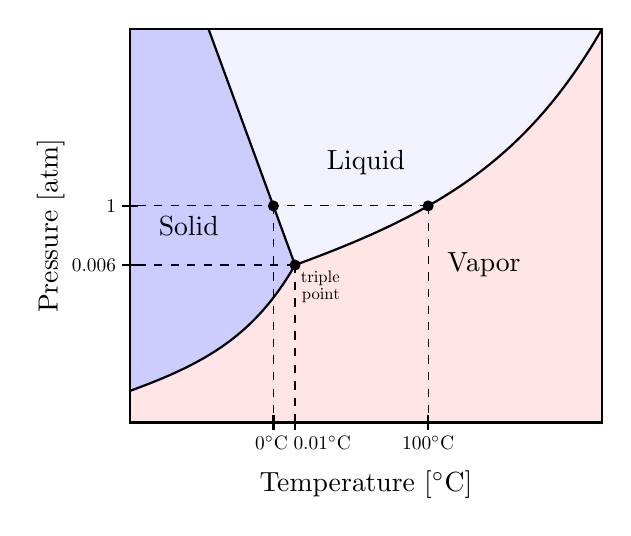
\begin{tikzpicture}[scale=0.5]
      \def\xtick#1#2{\draw[thick] (#1)++(0,.2) --++ (0,-.4) node[below=-.5pt,scale=0.7] {#2};}
      \def\ytick#1#2{\draw[thick] (#1)++(.2,0) --++ (-.4,0) node[left=-.5pt,scale=0.7] {#2};}
      
      % COORDINATES
      \coordinate (O) at (0,0);
      \coordinate (Q) at (0,0.8);
      \coordinate (N1) at (2,10);
      \coordinate (N2) at (11,10);
      \coordinate (NE) at (12,10);
      \coordinate (NW) at (0,10);
      \coordinate (SE) at (12,0);
      \coordinate (W) at (0,5);
      \coordinate (S) at (6,0);
      \coordinate (C) at (12,10); % critical
      \coordinate (T) at (4.2,4); % triple
      
      % PATHS
      \def\SL{(T) -- (N1)}
      \def\SG{(Q) to[out=20,in=-120] (T)}
      \def\LG{(T) to[out=20,in=-120] (C)}
      \def\atm{(0,5.5) -- (12,5.5)}
      \path[name path=SL] \SL;
      \path[name path=LG] \LG;
      \path[name path=atm] \atm;
      
      % REGIONS
      \fill[mylightblue] \SG -- (N1) -- (NW) -- cycle;
      \fill[blue!5] \LG -- (N2) -- (N1) -- cycle;
      \fill[mylightred] \LG -- (N2) -- (NE) -- (SE) -- (O) --  \SG -- cycle;
      \node at (1.5,5) {Solid};
      \node at (9,4) {Vapor};
      \node at (6,6.6) {Liquid};
      
      %% MIXED
      %\shade[top color=mylightblue,bottom color=mylightred,shading angle=70]
      %  (10.4,7.7) -- (11.2,10) -- (10.8,10) -- (10.0,7.7) -- cycle;
      
      % POINTS
      \fill[black,name intersections={of=SL and atm,by=M}] (M) circle (4pt);
      \fill[black,name intersections={of=LG and atm,by=B}] (B) circle (4pt);
      \fill (T) circle (4pt) node[below right,scale=0.6,align=right] {triple\\[-2pt]point};

      
      % LINES
      \draw[thick] \SG;
      \draw[thick] \LG;
      \draw[thick] \SL;
      \draw[dashed] (M) -- ($(M |- 0,0)$) coordinate (Mx);
      \draw[dashed] (T) -- ($(T |- 0,0)$) coordinate (Tx);
      \draw[dashed] (T) -- ($(T -| 0,0)$) coordinate (Ty);
      \draw[dashed] (B) -- ($(B |- 0,0)$) coordinate (Bx);
      \draw[dashed] (B) -- ($(B -| 0,0)$) coordinate (By);

      
      % AXES
      \draw[thick] (O) rectangle (NE);
      \node[left=20pt,above,rotate=90] at (W) {Pressure [atm]};

      \node[below=14pt] at (S) {Temperature [\si{\degree C}]};
      \xtick{Mx}{\hspace{-2pt}0\si{\degree C}}
      \xtick{Tx}{\hspace{28pt}0.01\si{\degree C}}
      \ytick{Ty}{0.006}
      \xtick{Bx}{100\si{\degree C}}
      \ytick{By}{1}
    \end{tikzpicture}

\end{figure}
\begin{figure}[h]
    \centering
    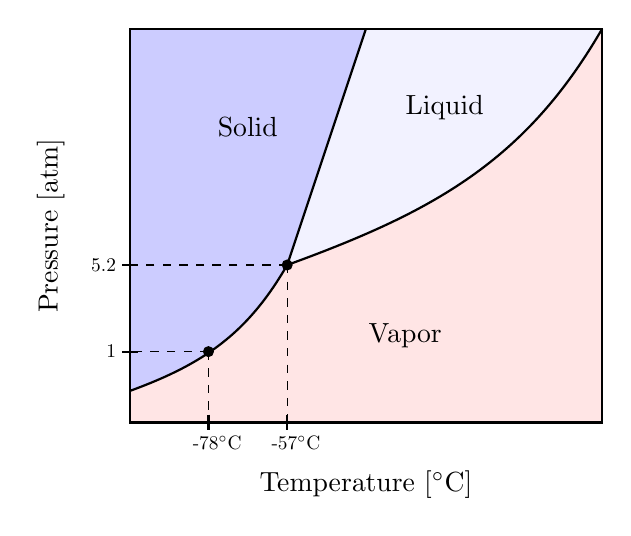
\begin{tikzpicture}[scale=0.5]
      \def\xtick#1#2{\draw[thick] (#1)++(0,.2) --++ (0,-.4) node[below=-.5pt,scale=0.7] {#2};}
      \def\ytick#1#2{\draw[thick] (#1)++(.2,0) --++ (-.4,0) node[left=-.5pt,scale=0.7] {#2};}
      
      % COORDINATES
      \coordinate (O) at (0,0);
      \coordinate (Q) at (0,.8);
      \coordinate (N1) at (6,10);
      \coordinate (N2) at (11,10);
      \coordinate (NE) at (12,10);
      \coordinate (NW) at (0,10);
      \coordinate (SE) at (12,0);
      \coordinate (W) at (0,5);
      \coordinate (S) at (6,0); 
      \coordinate (C) at (12,10); % critical
      \coordinate (T) at (4,4); % triple
      \coordinate (P) at (2,1.8);
      % PATHS
      \def\SL{(T) -- (N1)}
      \def\SG{(Q) to[out=20,in=-120] (T)}
      \def\LG{(T) to[out=20,in=-120] (C)}
      \def\atm{(0,5.5) -- (12,5.5)}
      \path[name path=SL] \SL;
      \path[name path=LG] \LG;
      \path[name path=atm] \atm;
      
      % REGIONS
      \fill[mylightblue] \SG -- (N1) -- (NW) -- cycle;
      \fill[blue!5] \LG -- (N2) -- (N1) -- cycle;
      \fill[mylightred] \LG -- (N2) -- (NE) -- (SE) -- (O) --  \SG -- cycle;
      \node at (3,7.5) {Solid};
      \node at (7,2.2) {Vapor};
      \node at (8,8) {Liquid};
      
      %% MIXED
      %\shade[top color=mylightblue,bottom color=mylightred,shading angle=70]
      %  (10.4,7.7) -- (11.2,10) -- (10.8,10) -- (10.0,7.7) -- cycle;
      
      % POINTS
      \fill (T) circle (4pt) node[below right,scale=0.6,align=right] {};
      \fill (P) circle (4pt) node[below right,scale=0.6,align=right] {};
      
      % LINES
      \draw[thick] \SG;
      \draw[thick] \LG;
      \draw[thick] \SL;
      \draw[dashed] (T) -- ($(T |- 0,0)$) coordinate (Tx);
      \draw[dashed] (T) -- ($(T -| 0,0)$) coordinate (Ty);
      \draw[dashed] (P) -- ($(P |- 0,0)$) coordinate (Px);
      \draw[dashed] (P) -- ($(P -| 0,0)$) coordinate (Py);
      
      % AXES
      \draw[thick] (O) rectangle (NE);
      \node[left=20pt,above,rotate=90] at (W) {Pressure [atm]};

      \node[below=14pt] at (S) {Temperature [\si{\degree C}]};
      \xtick{Tx}{\hspace{9pt}-57\si{\degree C}}
      \ytick{Ty}{5.2}
      \xtick{Px}{\hspace{9pt}-78\si{\degree C}}
      \ytick{Py}{1}
    \end{tikzpicture}

\end{figure}
The melting point of ice is lowered by increasing the pressure; so the curve has a \textbf{negative slope} - an unusual property of water. This is because ice has a lower density than that of pure water.

\end{document}